\documentclass[10pt, oneside]{article}   	
\usepackage[margin=0.8in]{geometry}  
\usepackage[dvips]{graphics}
\usepackage{epsfig}
\usepackage{amsmath}
\usepackage{xspace}
\usepackage{fancybox}
\usepackage{graphicx,xspace,cite,verbatim,comment}
\usepackage{mathtools,rotating,amsmath,amssymb}
\usepackage{color,cite,ifpdf,fancyvrb,array,listings}
\usepackage{algorithm,algpseudocode}
\usepackage{tabularx}


%SetFonts

%SetFonts


\title{\textbf{Stage5 Data Analysis}}
\author{Zhiwei Fan\hspace{7ex}
	   Lingfeng Huang\hspace{7ex}
	   Fang Wang\\
	   zfan29@wisc.edu\hspace{3ex}
	   lhuang58@wisc.edu\hspace{3ex}
	   fwang64@wisc.edu
	   }
%\date{}							% Activate to display a given date or no date

\begin{document}
\maketitle 

\section*{Term explanation}
\textit{tableA}: book data obtained from Barnes and Noble.\\ 
\textit{tableB}: book data obtained from Good reads. \\ 
\textit{scheme of both tables}: id, title,	authors, ISBN13,	pages,	publisher,	publishedYear,  publishedMonth, publishedDay\\
\textit{tableC}: the table after blocking stage.\\ 
\textit{tableE}: the table after merging stage. It has the same schema as tableA and tableB, but its id is not obtained from tableA nor tableB. Its id is new and in increasing order start from 0.

\section*{Description of table merging}
During the project stage 4, we chose \textit{random forest} as our final selected model because of its high F1 score.  
Thus, in this final stage, we first obtained the prediction result from running \textit{random forest} to the blocking tableC from stage4 (matching tuple pairs with information from tableA and tableB). By looking at the prediction boolean array generated from random forest, we generate a intermediate table containing tuple pairs that are predicted to be matched. We call this filtered-table. Our goal of merging is to ensure we find all unique tuples from tableA and tableB so we need to use this filtered-table in the next stage.

\subsubsection*{\textit{how did we generate merged table?}}
To generate tableE, we first keep all the data from tableA (always select the values from the tuple from table A) because tableA has well formatted data and there are lots of missing data in tableB. Thus, when there is a match, tableA's data has higher priority than data in tableB. After this step, we still have't added the tuples that are not present in tableA but present in tableB. Then, using the filtered-table from the last step, we are able to know which tuples in tableB have already presented in the tableA. We don't need these data so we take tableB and find all tuples which IDs are not  present in the filtered-table. These are the tuples that are not present in tableA but present in tableB. By adding these tuples to tableE as well, we have a complete tableE. During the process of adding tuples from tableB, we encountered several value misplacement issues: tableB has lots of dirty data in pages, publishedYear and publishedMonth field. For example,  value in pages is a publisher string instead of a number or value in publishedYear is misplaced by the author strings etc. For cases like this, we choose to discard these tuples since these tuples cannot be populated by finding matches in tableA. We also cleaned tableE so that in column id, title, pages, publishedYear, publishedMonth are having no misssing values (while ISBN13 may has missing value which is listed below in one of the sample from tableE). In summary, the step of merging is as follows: put all tuples from tableA to tableE, add tuples from tableB that has not yet been presented in the tableA into tableE as well. Perform some data cleaning while adding.

\subsubsection*{\textit{Statistics on Table E}}
\textbf{schema of table E}:   id, title,	authors, ISBN13,	pages,	publisher,	publishedYear,  publishedMonth, publishedDay\\
\textbf{number of tuples in table E}: 5922\\
\begin{table}[H]
\begin{tabular}{c}
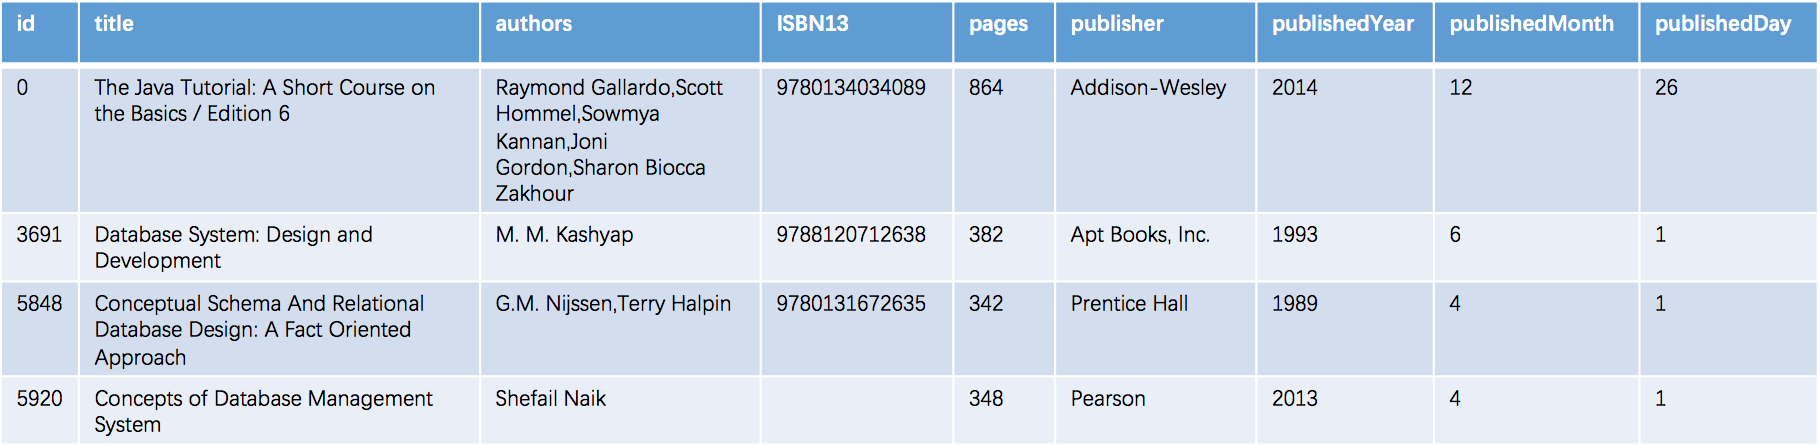
\includegraphics[width=16cm, height=4cm]{samples}
\end{tabular}
\caption{4 samples from tableE}
\end{table}

\section*{Data analysis}
Since our schema is quite simple and unfortunately we did not obtain the data of book prices nor user reviews, there are limited tasks we can do. We finally chose two data analysis tasks we would like to perform. First, we would like to know if the number of published books are increasing over the periods. Second, we would like to know if books are getting thicker (more pages) over the time periods.
\subsection*{\textit{Were there any problems with the analysis process and with the data?}}
To conduct data analysis, we performed clustering based on grouping all tuples by its published periods (10 year per period), then we counted the number of books published in the periods and also calculate the average pages for each period. In the first iteration, we found that the average of pages are abnormally high in some periods. Thus, we perform anomaly detection by first sorting fields including pages, publishedYear and publishedMonth, we detected books that have over 20,000 pages which are obviously wrong and we also detected publishedMonth that has value of 1996 which seems to be a duplication of its publishedYear. We cleaned the abnormal data and luckily these unusual cases are small so deleting these tuples would not create biased clustering result. (the 5922 tuples in tableE are the tuples survived after this process)\\
After anomaly detection and further data cleaning. We performed clustering again. This time the result are as follows (Note that the time periods are represented by their first year, here 1960 means the period from 1960 to 1970 instead of a single year):

\begin{table}[H]
\centering
\begin{tabular}{c}
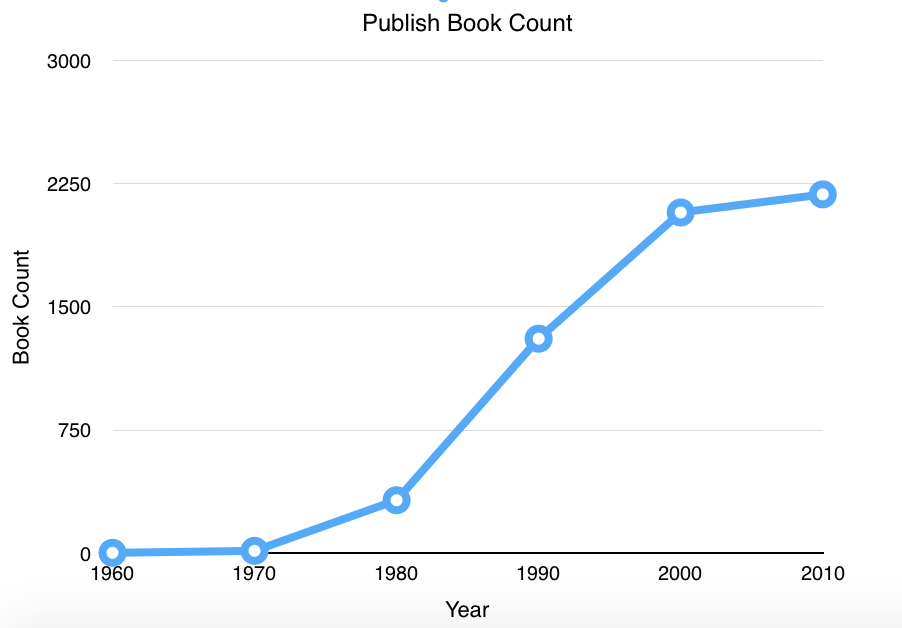
\includegraphics[width=12cm, height=8cm]{bookcount}
\end{tabular}
\caption{relation between book counts and published periods}
\end{table}

\begin{table}[H]
\centering
\begin{tabular}{c}
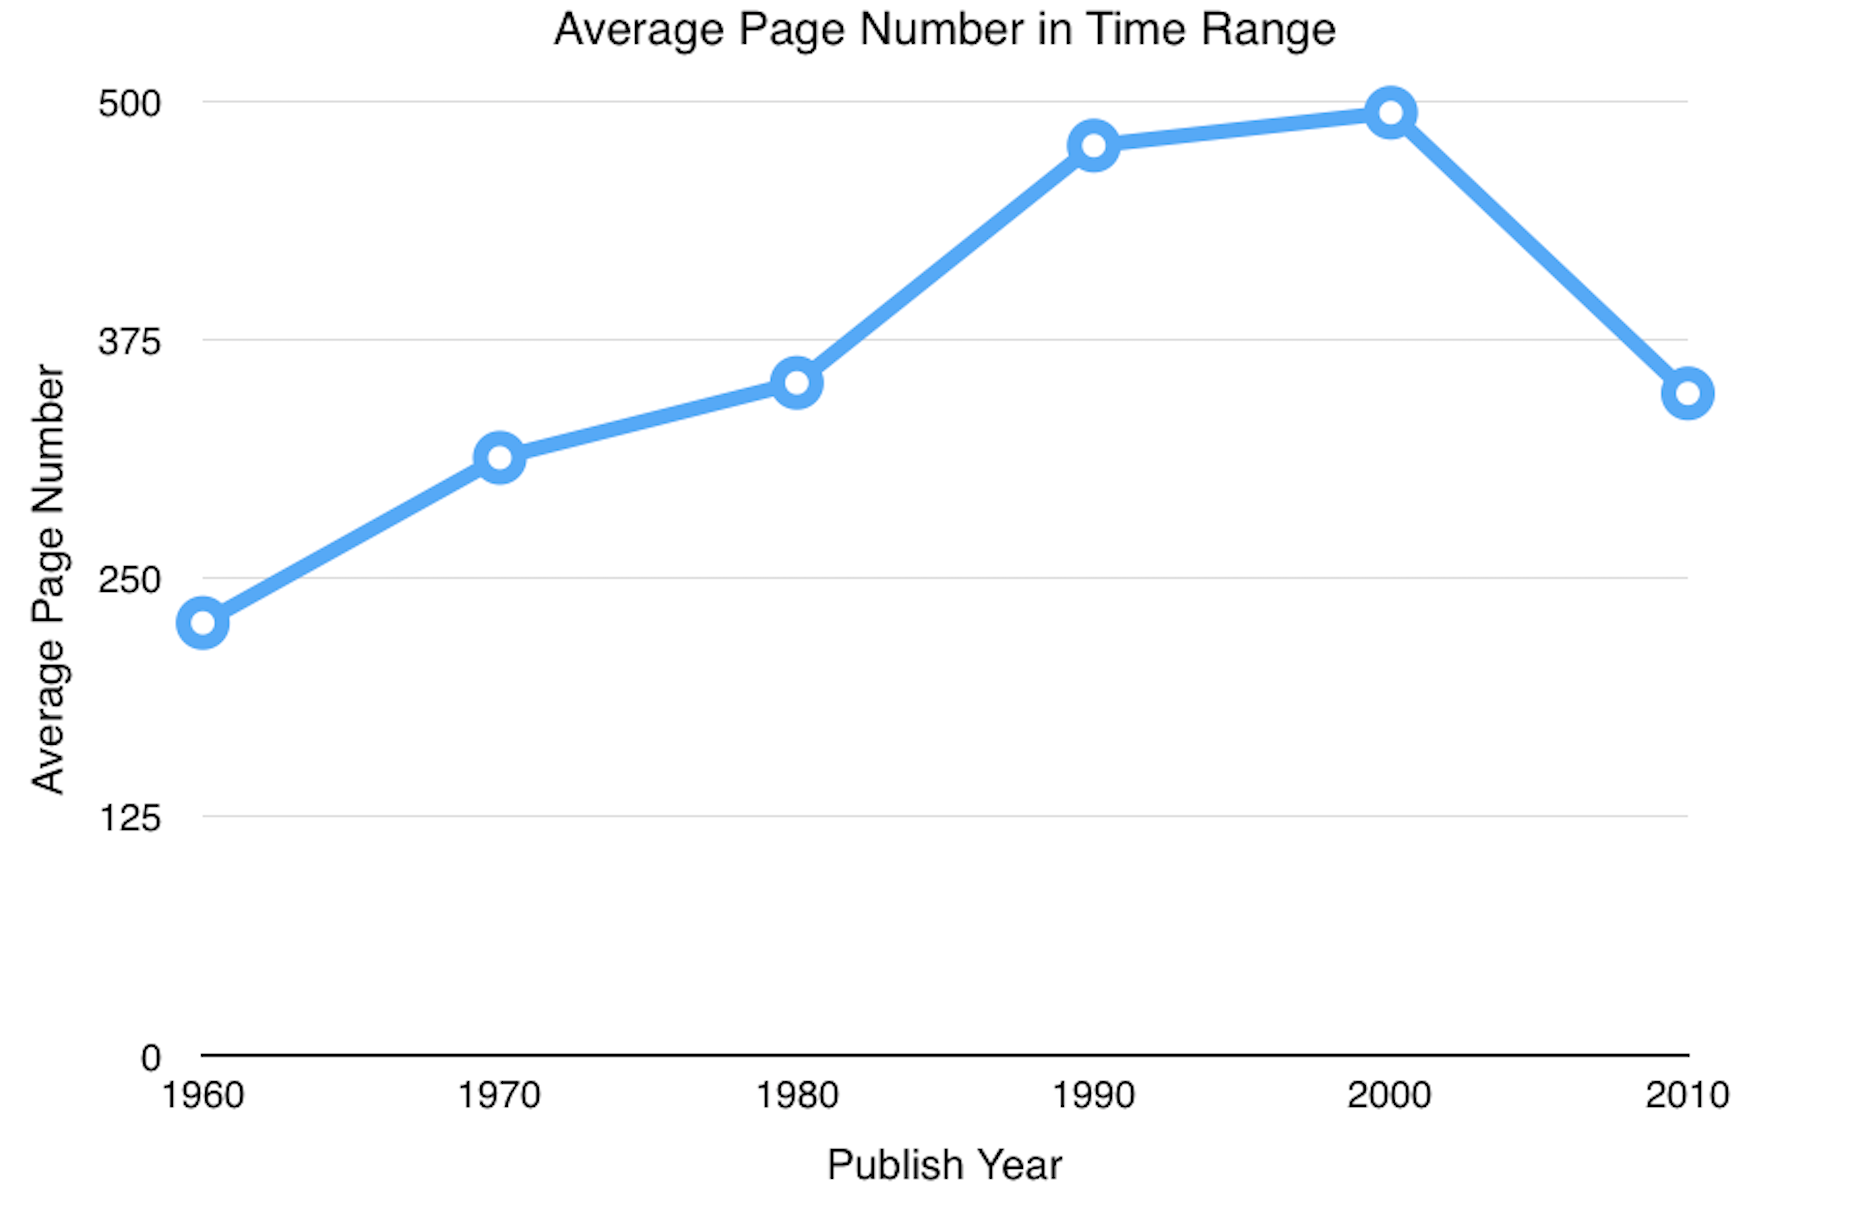
\includegraphics[width=12cm, height=8cm]{average}
\end{tabular}
\caption{relation between pages and published periods}
\end{table}

\section*{Discussion}
\subsubsection*{\textit{What did we learn/conclude from our data analysis?  }}
From table2, we can clearly see a rise in pages of books from time periods started from 1960-1970 period. This proves our first data analysis assumption. Thus, we expect in the future the number of published books will continue to increase. However, from table3, although the average book pages are steadily increases from 1960s to 2000s, the average book pages decrease since 2010. After our discussion, we think 500 pages might be the threshold for a author to choose to write more books (or a series of books) instead of write one thick book that has everything. Furthermore, we also think that the increasing competition from online study resources could also be a factor that decreases the motivation for a author to write a thick book. The authors may choose to write thinner book that does not include older knowledges since these parts may already be posted free online. The increasing number of published book also supports this assumption.  These are just our assumptions from our limited data.

\subsubsection*{\textit{What we do next}}
We realised that our schema is too simple to go through complicated data analysis. Thus, if possible, we may try adding prices or user reviews to our schema so we can have more correlations to perform data analysis. Besides new data, we can also fill out some missing values in ISBN13 for some books. 

\end{document}  